\documentclass[10pt,letterpaper,twocolumn]{article}

\usepackage[margin=0.75in]{geometry}
\usepackage{times}
\usepackage{microtype}
\usepackage{graphicx}
\usepackage{booktabs}
\usepackage{xcolor}
\usepackage{hyperref}
\usepackage{caption}
\usepackage{tikz}
\usepackage{pgfplots}
\pgfplotsset{compat=1.18}
\usetikzlibrary{shapes.geometric, arrows.meta, positioning, fit, backgrounds}

\hypersetup{colorlinks=true, urlcolor=blue!60!black, linkcolor=black, citecolor=black}
\setlength{\columnsep}{0.25in}
\setlength{\parskip}{2pt}
\setlength{\parindent}{0pt}

\title{\vspace{-1.5em}Progress Report: An Agent-Routed, Memory-Augmented\\
Annotation Workflow for Biomedical Segmentation}
\author{Shuheng (Andy) Cao \\ \small{\texttt{s8cao@ucsd.edu}}}
\date{}

\begin{document}
\maketitle
\vspace{-1.8em}

\section{Problem and Goal}
Biomedical segmentation tools fall into two camps that rarely meet in
the same workflow: \emph{interactive editors} (3D~Slicer, ITK-SNAP,
QuPath) that give clinicians fine manual control but no model-assisted
priors, and \emph{model-centric pipelines} (MedSAM, MedSAM2, LangSAM,
Cellpose) that produce strong masks but offer little transparency,
auditability, or reuse of prior prompts. The result is annotation
sessions in which the user cannot see \emph{why} a particular backend
was chosen, cannot reuse a useful bbox or text prompt across similar
slices, and cannot reproduce a session from its exported masks.

This project builds a lightweight desktop and headless workflow that
combines manual contouring, classical baselines, and optional
foundation-model backends behind a single API, with three properties
that distinguish it from existing tools: (1)~a transparent
\emph{agentic router} that selects a backend from prompt and image
cues and logs its reasoning; (2)~a \emph{geometry memory} that
suggests prior prompts/masks without overwriting user edits; and
(3)~per-session \emph{provenance sidecars} so every exported mask
carries its route, runtime, and prompt context.

\section{Progress Since Proposal}

\subsection{System architecture is implemented end-to-end}

The full software path runs today in lightweight mode (no heavy
checkpoints required). Figure~\ref{fig:arch} shows the realised
architecture; every block in the diagram corresponds to a working
Python module in the repository (66 source files, 17 test modules,
\texttt{pytest -q} passing on Windows~11/Python~3.11).

\begin{figure}[t]
\centering
\resizebox{\columnwidth}{!}{%
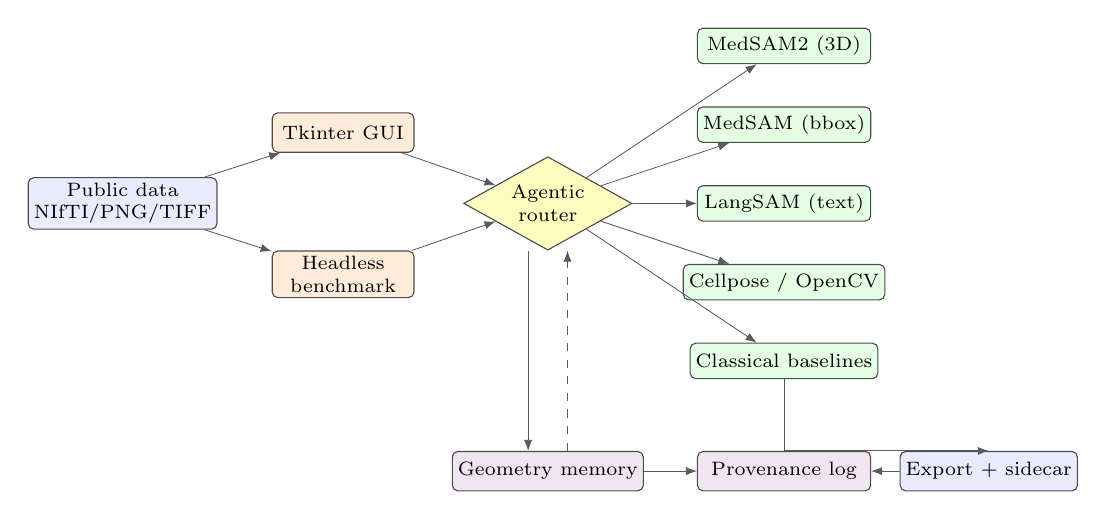
\begin{tikzpicture}[
  font=\scriptsize,
  every node/.style={align=center, inner sep=2pt},
  io/.style      ={rectangle, rounded corners=2pt, draw=black!70, fill=blue!8,    minimum height=5mm, minimum width=18mm},
  ui/.style      ={rectangle, rounded corners=2pt, draw=black!70, fill=orange!15, minimum height=5mm, minimum width=18mm},
  router/.style  ={diamond, aspect=1.8, draw=black!70, fill=yellow!25, minimum height=8mm, minimum width=14mm},
  backend/.style ={rectangle, rounded corners=2pt, draw=black!70, fill=green!10,  minimum height=4.5mm, minimum width=22mm},
  store/.style   ={rectangle, rounded corners=2pt, draw=black!70, fill=violet!10, minimum height=5mm,  minimum width=22mm},
  arr/.style     ={-{Latex[length=1.4mm]}, draw=black!65, line width=0.3pt}
]
% Grid coordinates: x in cm (col), y in cm (row)
% Col 1 (x=0): input data
\node[io] (data) at (0,0) {Public data \\ NIfTI/PNG/TIFF};

% Col 2 (x=2.6): UI / headless stacked vertically with safe gap
\node[ui] (gui)      at (2.8, 0.9) {Tkinter GUI};
\node[ui] (headless) at (2.8,-0.9) {Headless\\benchmark};

% Col 3 (x=5.4): router
\node[router] (router) at (5.4,0) {Agentic\\router};

% Col 4 (x=8.4): backends stacked with 8mm vertical gap
\node[backend] (medsam2)   at (8.4, 2.0)  {MedSAM2 (3D)};
\node[backend] (medsam)    at (8.4, 1.0)  {MedSAM (bbox)};
\node[backend] (langsam)   at (8.4, 0.0)  {LangSAM (text)};
\node[backend] (cellpose)  at (8.4,-1.0)  {Cellpose / OpenCV};
\node[backend] (classical) at (8.4,-2.0)  {Classical baselines};

% Bottom row (y = -3.4): memory directly under router, then prov, export to the right
\node[store] (memory) at (5.4,-3.4) {Geometry memory};
\node[store] (prov)   at (8.4,-3.4) {Provenance log};
\node[io]    (export) at (11.0,-3.4) {Export + sidecar};

% Edges
\draw[arr] (data)     -- (gui);
\draw[arr] (data)     -- (headless);
\draw[arr] (gui)      -- (router);
\draw[arr] (headless) -- (router);
\draw[arr] (router)   -- (medsam2);
\draw[arr] (router)   -- (medsam);
\draw[arr] (router)   -- (langsam);
\draw[arr] (router)   -- (cellpose);
\draw[arr] (router)   -- (classical);
% Pure-vertical router <-> memory pair, two parallel arrows
\draw[arr]         ([xshift=-2.5mm]router.south) -- ([xshift=-2.5mm]memory.north);
\draw[arr, dashed] ([xshift=2.5mm]memory.north)  -- ([xshift=2.5mm]router.south);
% Memory feeds prov as well
\draw[arr] (memory) -- (prov);
\draw[arr] (classical.south) |- (export.north);
\draw[arr] (export) -- (prov);
\end{tikzpicture}}
\caption{Implemented architecture. Solid arrows are runtime calls;
the dashed arrow is the memory$\rightarrow$router suggestion path.
Heavy backends (MedSAM/MedSAM2/LangSAM) are accessed via external
command bridges so the lightweight install runs without a GPU.}
\label{fig:arch}
\end{figure}

Concretely, the following pieces are working and exercised by tests:

\begin{itemize}
  \setlength{\itemsep}{1pt}
  \item \textbf{Unified backend API} (\texttt{segmentation/backends/})
    with mock, classical (OpenCV watershed/levelset), Cellpose, and
    external-bridge wrappers for LangSAM, MedSAM, MedSAM2.
  \item \textbf{Deterministic agentic router}
    (\texttt{agent/router.py}, \texttt{agent/workflow.py}) that ranks
    candidate backends from prompt tokens, image dimensionality, and
    bbox/seed presence, and emits a structured
    \texttt{RoutingDecision} record (selected backend, ranked list,
    fallback history, prompt interpretation).
  \item \textbf{Memory store} (\texttt{memory/}) that records prompt
    geometry and result summaries without raw pixels by default, so
    sessions can be reused across similar slices.
  \item \textbf{Provenance sidecars}
    (\texttt{provenance/}) and a \texttt{python -m
    app.provenance.inspect} CLI for review.
  \item \textbf{Headless benchmark runner}
    (\texttt{benchmarks/run\_benchmark.py}) that emits
    \texttt{metrics.csv}, \texttt{routing\_decisions.jsonl},
    per-case provenance, and \texttt{report.md}.
  \item \textbf{Tkinter GUI} (\texttt{python\_app/main.py}) that
    routes through the same workflow and was launched and verified
    on the development machine.
\end{itemize}

\subsection{Resources secured}

LaTeX/MiKTeX, Python 3.11, OpenCV, NumPy/SciPy, and Cellpose are
installed locally; per-backend isolated environments live under
\texttt{.model\_envs/cellpose/} and \texttt{.model\_envs/langsam/}
to keep heavy dependencies off the main interpreter. Public dataset
targets are scoped (MSD subset for 3D~medical, Cellpose/BBBC for
microscopy) with manifest schemas checked by
\texttt{app.configs.validate} and a preflight gate
(\texttt{app.experiments.preflight}) that refuses to launch a real
benchmark unless paths, masks, and licenses are present.

\subsection{Working GUI prototype}

Figure~\ref{fig:gui} is a screenshot of the running Tkinter annotator
(\texttt{python python\_app/main.py}) on the development machine. The
left panel exposes file I/O, the five export formats wired up so far
(PNG, NIfTI, TIFF, polygon JSON, COCO JSON), intensity windowing /
slice navigation, and four tool tabs --- manual contouring, classical
watershed, level-set, and the \emph{AI~Agent} tab that calls into the
router shown in Fig.~\ref{fig:arch}. The session-log line under
``Files'' is the per-session provenance JSONL emitted automatically.

\begin{figure}[t]
\centering
\fbox{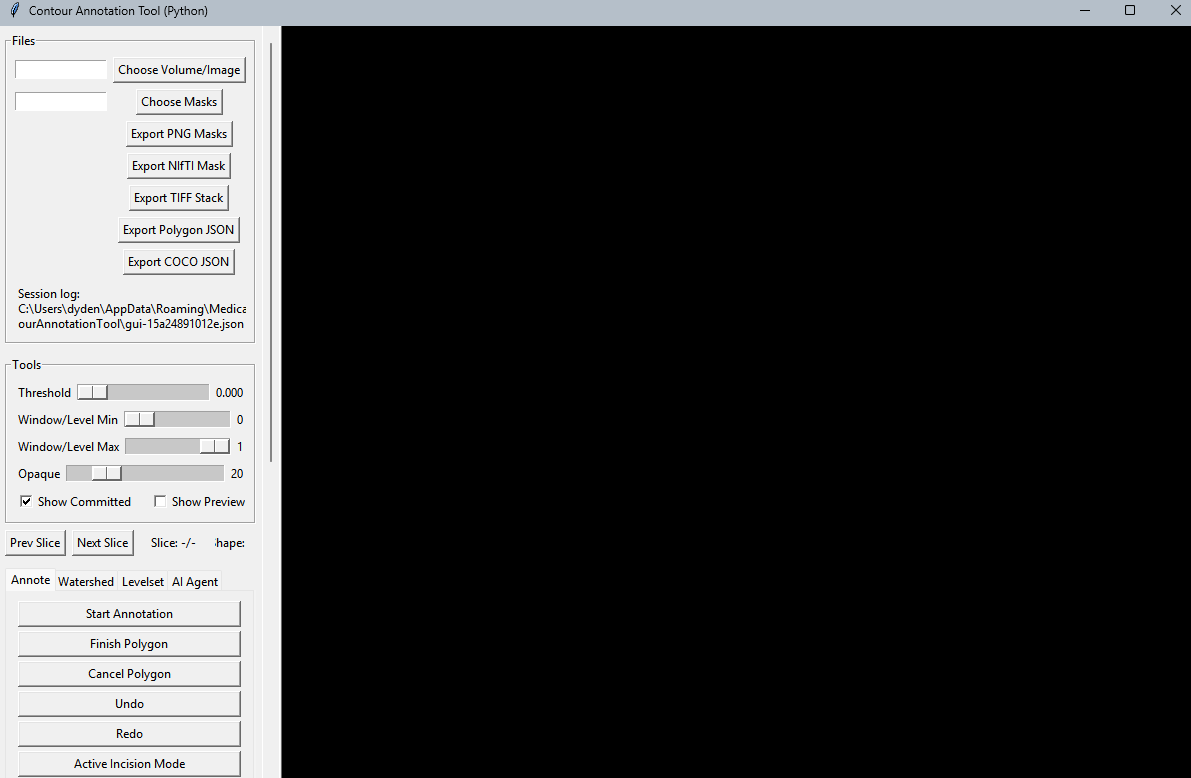
\includegraphics[width=\columnwidth]{figures/gui_screenshot.png}}
\caption{Live Tkinter annotator launched on May~12, 2026. Left
column: file I/O, multi-format mask export (PNG / NIfTI / TIFF /
polygon JSON / COCO JSON), the auto-generated session-log path,
intensity / window-level / slice tools, and tool tabs (Annotate /
Watershed / Levelset / AI~Agent). The dark region on the right is
the image canvas before a volume is loaded.}
\label{fig:gui}
\end{figure}

\subsection{Initial quantitative results (synthetic smoke only)}

Figure~\ref{fig:dice} reports Dice scores from the synthetic smoke
benchmark (the only quantitative results currently authorised by the
project's claim policy --- real public-dataset numbers remain
\texttt{NOT\_RUN}). The router correctly sends the 2D synthetic
microscopy case to the Cellpose backend and the 3D synthetic organ
case to the classical fallback, demonstrating that prompt/image cues
flow through the router into backend selection as designed. The
mock-only ablation isolates router overhead and confirms the routing
layer adds $<\!1$\,ms per case.

\begin{figure}[t]
\centering
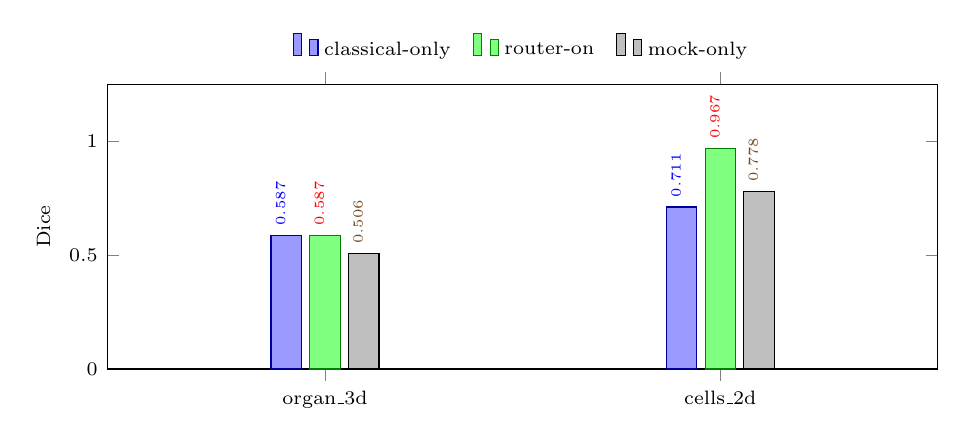
\begin{tikzpicture}
\begin{axis}[
  width=\columnwidth, height=5.2cm,
  ybar=3pt, bar width=11pt,
  ymin=0, ymax=1.25,
  ylabel={Dice}, ylabel near ticks,
  symbolic x coords={organ\_3d, cells\_2d},
  xtick=data,
  enlarge x limits=0.55,
  legend style={font=\scriptsize, at={(0.5,1.20)}, anchor=north,
                legend columns=3, draw=none,
                /tikz/every even column/.append style={column sep=6pt}},
  tick label style={font=\scriptsize},
  label style={font=\scriptsize},
  nodes near coords,
  nodes near coords style={font=\tiny, rotate=90, anchor=west,
                           xshift=0pt, yshift=2pt},
  every node near coord/.append style={/pgf/number format/fixed,
                                       /pgf/number format/precision=3},
]
\addplot+[fill=blue!40,  draw=blue!60!black]   coordinates {(organ\_3d, 0.5869) (cells\_2d, 0.7109)};
\addplot+[fill=green!50, draw=green!50!black]  coordinates {(organ\_3d, 0.5869) (cells\_2d, 0.9668)};
\addplot+[fill=gray!50,  draw=black]           coordinates {(organ\_3d, 0.5060) (cells\_2d, 0.7777)};
\legend{classical-only, router-on, mock-only}
\end{axis}
\end{tikzpicture}
\caption{Synthetic smoke Dice from
\texttt{results/synthetic\_smoke/metrics.csv} and
\texttt{results/mock\_ablation/}. Router-on selects \textsc{cellpose}
for the 2D microscopy case (Dice 0.967) and \textsc{classical} for
the 3D organ case (Dice 0.587), matching the routing rules in
\texttt{agent/router.py}. Numbers are software-path validation, not
biomedical accuracy claims.}
\label{fig:dice}
\end{figure}

\section{What Remains}

The engineering scaffold is in place; the remaining work is
\emph{evidence}, not infrastructure. Concrete next steps, in order:
(1)~download the MSD~Spleen subset and one Cellpose split, fill
\texttt{configs/datasets.local.yaml}, and run the real-data
benchmark templates already wired up; (2)~run baseline exports from
3D~Slicer and Cellpose using the protocols in
\texttt{baseline\_protocols/} for a head-to-head comparison;
(3)~execute the brief usability/time pilot
(\texttt{docs/usability\_study\_protocol.md}) on $3$--$5$ users; and
(4)~produce the camera-ready architecture and results figures from
the same scaffolds used here.

\paragraph{Risks.} The largest remaining risk is heavy-backend setup
on a machine with limited GPU memory; the bridge protocol
(\texttt{.npy} in / \texttt{.npy} out, JSON request file) was chosen
specifically so the GUI keeps working when a checkpoint is missing,
and the synthetic smoke path validates the router/memory/provenance
layers independently of any model weights.

\end{document}
